\subsection{Nernst-Plank Equation}
\label{appendixNPE}
Ion flux across a membrane can be described by the Nernst-Plank equation. For an ion, $K$, with valance charge, $z$, the total flux can be described as the sum of the contributions of the diffusion flux $J_{diff}$ and the electric flux $J_{elec}$. $J_{diff}$ can be described by Fick's law:
\begin{equation}
    J_{diff} = -D\nabla c
\end{equation}
where $D$ is the diffusion coefficient and $c$ is the concentration of the ion. $J_{elec}$ satisfies the Plank equation:
\begin{equation}
    J_{elec} = -\frac{z}{|z|}\mu c\nabla u
\end{equation}
where $\frac{z}{|z|}$ is $+1$ for positive ions and $-1$ for negative ions, $\mu$ is the mobility of the ion and $u$ is the electric potential. \par

In both cases the ion mobility is inhibited by the presence of the solvent, as such Einstein \citep{einstien} found that $D$ and $\mu$ are related:
\begin{equation}
    D = \frac{\mu RT}{|z|F}
\end{equation}
where $R$ is the ideal gas constant, $T$ is temperature and $F$ is Faraday's constant. It follows that:
\begin{equation}
    J_{total} = J_{diff}+J_{elec} = -D\bigg(\nabla c + \frac{zF}{RT}c\nabla u\bigg)
    \label{nerstplankeq}
\end{equation}
which is known as the Nernst-Plank equation.

\subsection{Goldman-Hodgkin-Katz Current-Voltage Relation}
\label{appendixGHK}
Upon assuming $J$ and $u$ are transverse to the membrane, equation \ref{nerstplankeq} can be transformed into a linear differential equation in one dimension. 
\begin{equation}
    \frac{dc}{dx}(x)+\frac{zF}{RT}\frac{du}{dx}(x)c(x)+\frac{J}{D} = 0
\end{equation}
The solution to this can be found by multiplying by an exponential and intergrating. By then assuming the electric field is constant across the membrane of length $L$ and by using the result of the one dimensional Nernst-Plank equation the following relation can be found:
\begin{equation}
    c(x) = \frac{JRTL}{DzvF}\bigg(1-exp\bigg(\frac{zvF}{RTL}x\bigg)\bigg)+c^iexp\bigg(\frac{zvF}{RTL}x\bigg)
\end{equation}
where $v = u(0)-u(L) = u_i-u_e$. $i$ and $e$ notation is used to indicate intra and extracellular values. $c(0) = c^i$ so to satisfy $c(L) = c^e$ it follows that 
\begin{equation}
    J = \frac{DzFv}{LRT}\frac{c^i-c^eexp\big(\frac{-zvF}{RT}\big)}{1-exp\big(\frac{-zvF}{RT}\big)}
\end{equation}
By defining the electric current density $I := zFJ$ the Goldman-Hodgkin-Katz (GHK) relation is obtained.
\begin{equation}
    I=P\frac{z^2F^2}{RT}v\frac{c^i-c^eexp\big(\frac{-zvF}{RT}\big)}{1-exp\big(\frac{-zvF}{RT}\big)}
\end{equation}
where $P = \frac{D}{L}$ is the permeability of the membrane to the ion. The GHK relation is key to calculating the ion concentrations and currents discussed in section \ref{cellelectro}.

\subsection{Van Der Pol Relaxation Oscilator}
\label{appendixVDP}
First proposed in 1920 by Balthasar van der Pol, it is an oscillator with non-linear damping governed by a second order differential of the form
\begin{equation}
    \frac{dx^2}{d^2t}-\epsilon(1-x^2)\frac{dx}{dt}+x=0
\end{equation}
where $x$ is the dynamic variable (the parameter $\epsilon$ is $>0$). Using the transformation $y=x-(x^3/3)-(\frac{dx}{dt}/\epsilon)$, known as Liénard's transformation, the equation becomes
\begin{equation}
    \begin{split}
        & \frac{dx}{dt}=\epsilon(x-\frac{1}{3}x^3-y) \\
        & \frac{dy}{dt}=\frac{x}{\epsilon} \\
    \end{split}
\end{equation}
This is known as the Bonhoeffer-van der Pol model which can be electronically modelled as shown in figure \ref{fig3.2}. This circuit produces a relaxation oscillation with a period determined by the inductor and resistor. Further information can be found in the supporting literature \citep{vdp}.
\begin{SCfigure}[0.9][h!]
    \centering
    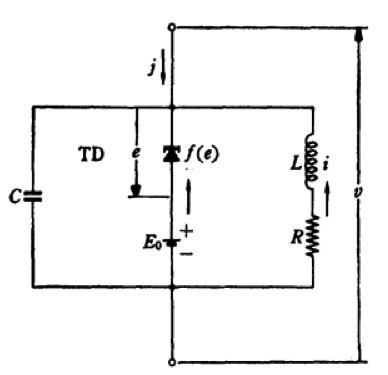
\includegraphics[width=0.4\textwidth]{images/BVP.png}
    \caption{A Bonhoeffer-Van der Pol electronic circuit, has a measured current (j) that acts as a Van der Pol relaxation oscillator. \citep{fitzhughnagumo}}
    \label{fig3.2}
\end{SCfigure}
These circuits can be coupled together to simulate a nurve axon.
\begin{SCfigure}[0.9][h!]
    \centering
    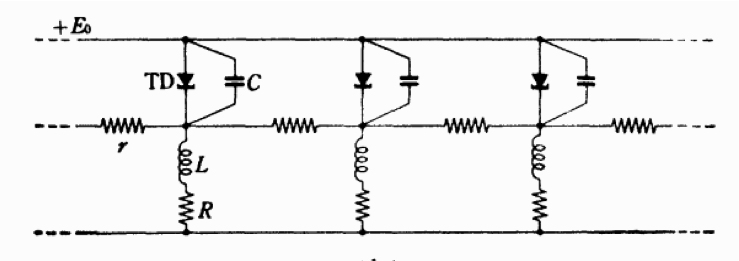
\includegraphics[width=0.7\textwidth]{images/FNaxon.png}
    \caption{A linear combination of BVP circuits (\ref{appendixVDP}) used to simulate signal propagation down a nerve axon. \citep{fitzhughnagumo}}
    \label{fig3.3}
\end{SCfigure}

\subsection{Electronic Circuit Model}
\label{appendixcircuit}
\begin{figure}[H]
    \centering
    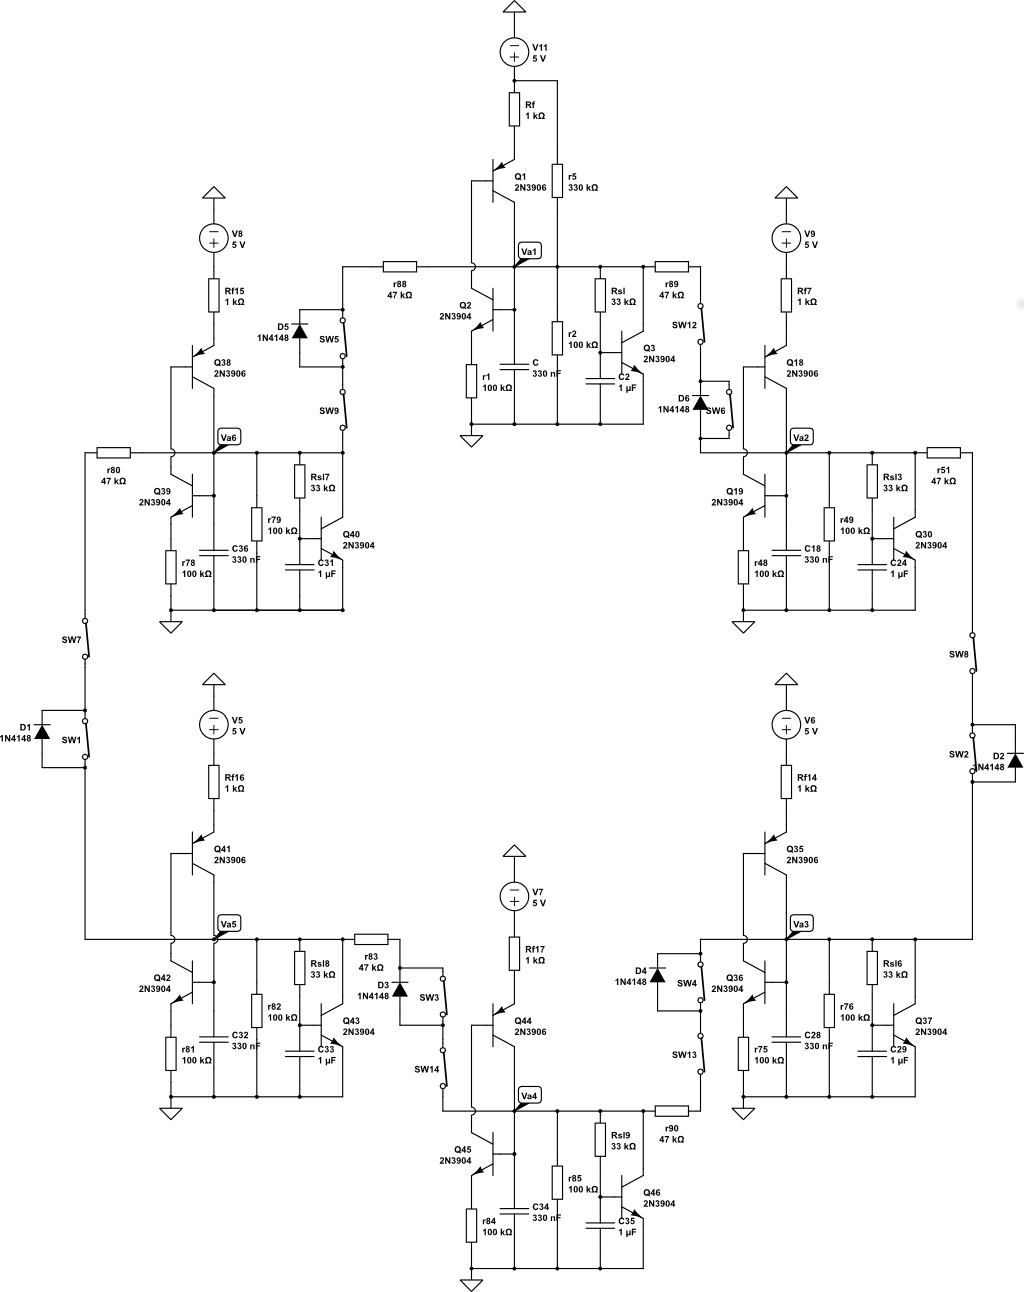
\includegraphics[width=0.9\textwidth]{images/full-circuit.png}
    \caption{A circuit diagram of 6 cells connected in a 2D ring.}
    \label{fig3.6}
\end{figure}
\begin{figure}[H]
    \centering
    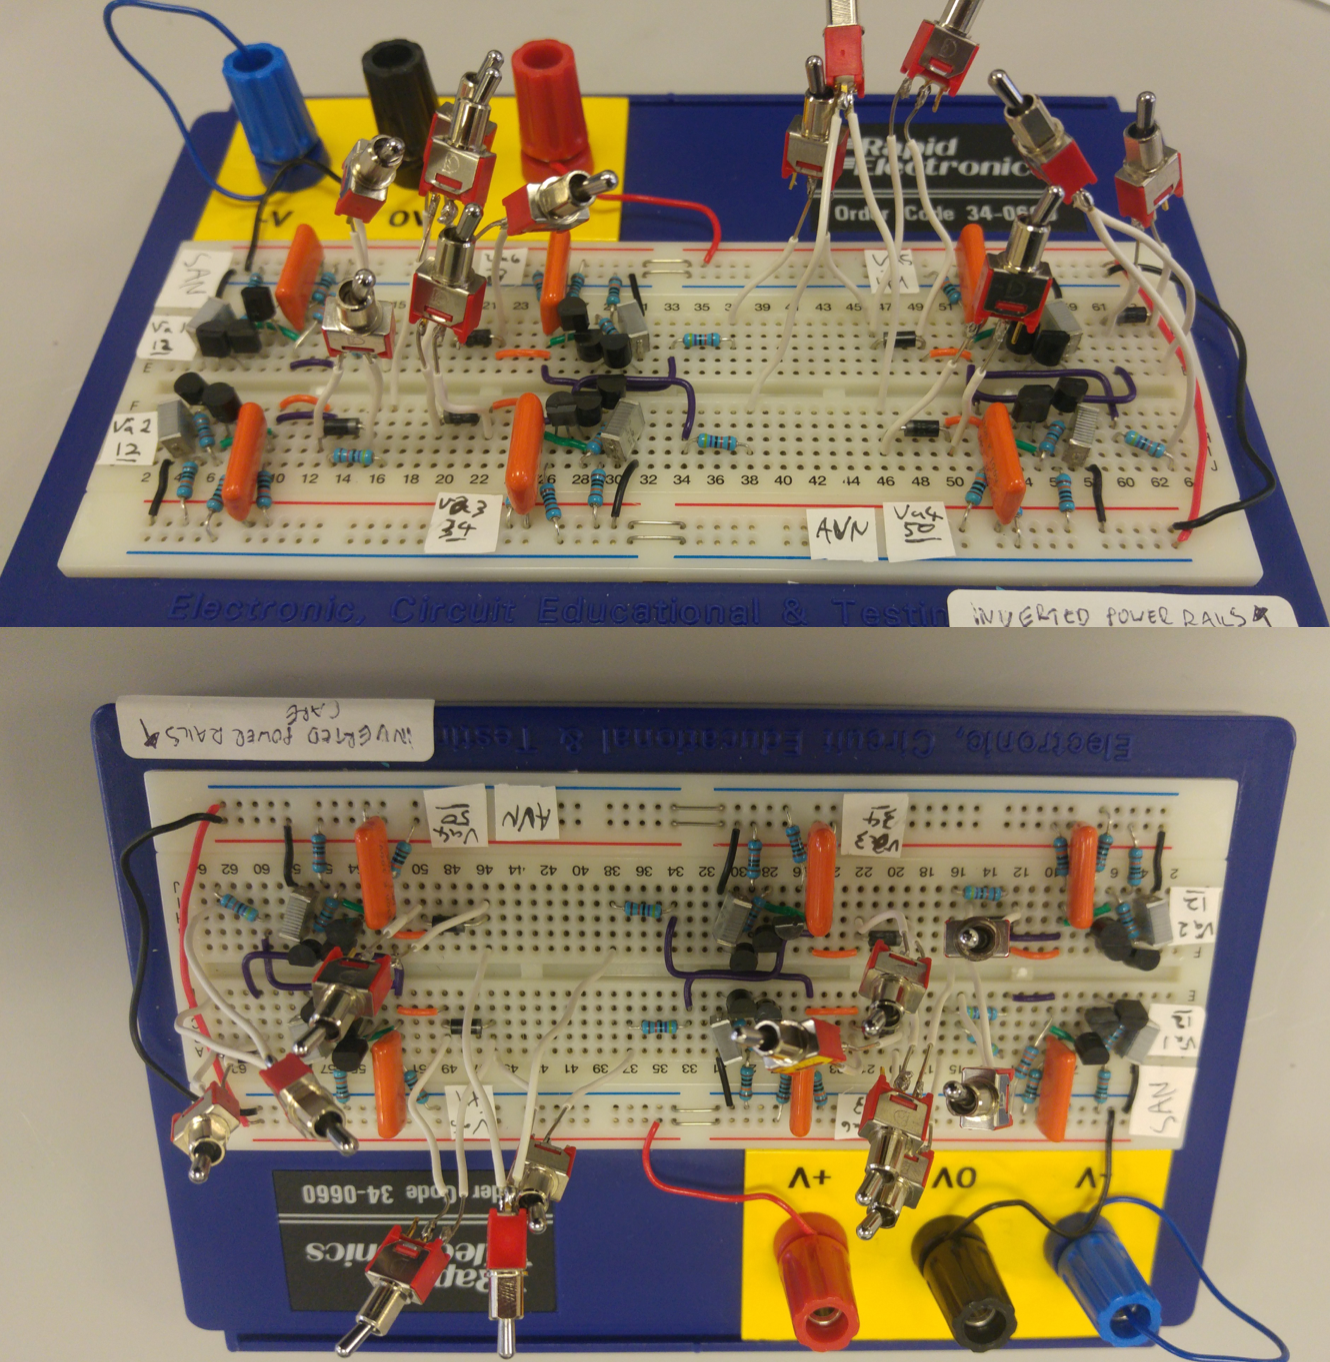
\includegraphics[width=\textwidth]{images/circuitappendix.png}
\end{figure}

\subsection{2D Code}
\label{appendix2D}
    \subsubsection{Main Code}
       \pythonexternal{main.py}
    \subsubsection{Parameters}
       \pythonexternal{param.py}
    \subsubsection{Grid Formation}
       \pythonexternal{gridCalc.py}
    \subsubsection{Solver}
       \pythonexternal{solvePlot.py}
    \subsubsection{Output Viewer}
       \pythonexternal{3dheatmap.py}

\subsection{3D Code}
\label{appendix3D}
To run the model in 3D simply add in an additional dimension to the matrix and a calculation path in the $z$ directions in the same way as $x$ and $y$ propagation are implemented.
    \subsubsection{3D Output viewer}
        \pythonexternal{4dheatmap.py}